% Options for packages loaded elsewhere
\PassOptionsToPackage{unicode}{hyperref}
\PassOptionsToPackage{hyphens}{url}
\documentclass[
]{article}
\usepackage{xcolor}
\usepackage[margin=1in]{geometry}
\usepackage{amsmath,amssymb}
\setcounter{secnumdepth}{-\maxdimen} % remove section numbering
\usepackage{iftex}
\ifPDFTeX
  \usepackage[T1]{fontenc}
  \usepackage[utf8]{inputenc}
  \usepackage{textcomp} % provide euro and other symbols
\else % if luatex or xetex
  \usepackage{unicode-math} % this also loads fontspec
  \defaultfontfeatures{Scale=MatchLowercase}
  \defaultfontfeatures[\rmfamily]{Ligatures=TeX,Scale=1}
\fi
\usepackage{lmodern}
\ifPDFTeX\else
  % xetex/luatex font selection
\fi
% Use upquote if available, for straight quotes in verbatim environments
\IfFileExists{upquote.sty}{\usepackage{upquote}}{}
\IfFileExists{microtype.sty}{% use microtype if available
  \usepackage[]{microtype}
  \UseMicrotypeSet[protrusion]{basicmath} % disable protrusion for tt fonts
}{}
\makeatletter
\@ifundefined{KOMAClassName}{% if non-KOMA class
  \IfFileExists{parskip.sty}{%
    \usepackage{parskip}
  }{% else
    \setlength{\parindent}{0pt}
    \setlength{\parskip}{6pt plus 2pt minus 1pt}}
}{% if KOMA class
  \KOMAoptions{parskip=half}}
\makeatother
\usepackage{graphicx}
\makeatletter
\newsavebox\pandoc@box
\newcommand*\pandocbounded[1]{% scales image to fit in text height/width
  \sbox\pandoc@box{#1}%
  \Gscale@div\@tempa{\textheight}{\dimexpr\ht\pandoc@box+\dp\pandoc@box\relax}%
  \Gscale@div\@tempb{\linewidth}{\wd\pandoc@box}%
  \ifdim\@tempb\p@<\@tempa\p@\let\@tempa\@tempb\fi% select the smaller of both
  \ifdim\@tempa\p@<\p@\scalebox{\@tempa}{\usebox\pandoc@box}%
  \else\usebox{\pandoc@box}%
  \fi%
}
% Set default figure placement to htbp
\def\fps@figure{htbp}
\makeatother
% definitions for citeproc citations
\NewDocumentCommand\citeproctext{}{}
\NewDocumentCommand\citeproc{mm}{%
  \begingroup\def\citeproctext{#2}\cite{#1}\endgroup}
\makeatletter
 % allow citations to break across lines
 \let\@cite@ofmt\@firstofone
 % avoid brackets around text for \cite:
 \def\@biblabel#1{}
 \def\@cite#1#2{{#1\if@tempswa , #2\fi}}
\makeatother
\newlength{\cslhangindent}
\setlength{\cslhangindent}{1.5em}
\newlength{\csllabelwidth}
\setlength{\csllabelwidth}{3em}
\newenvironment{CSLReferences}[2] % #1 hanging-indent, #2 entry-spacing
 {\begin{list}{}{%
  \setlength{\itemindent}{0pt}
  \setlength{\leftmargin}{0pt}
  \setlength{\parsep}{0pt}
  % turn on hanging indent if param 1 is 1
  \ifodd #1
   \setlength{\leftmargin}{\cslhangindent}
   \setlength{\itemindent}{-1\cslhangindent}
  \fi
  % set entry spacing
  \setlength{\itemsep}{#2\baselineskip}}}
 {\end{list}}
\usepackage{calc}
\newcommand{\CSLBlock}[1]{\hfill\break\parbox[t]{\linewidth}{\strut\ignorespaces#1\strut}}
\newcommand{\CSLLeftMargin}[1]{\parbox[t]{\csllabelwidth}{\strut#1\strut}}
\newcommand{\CSLRightInline}[1]{\parbox[t]{\linewidth - \csllabelwidth}{\strut#1\strut}}
\newcommand{\CSLIndent}[1]{\hspace{\cslhangindent}#1}
\setlength{\emergencystretch}{3em} % prevent overfull lines
\providecommand{\tightlist}{%
  \setlength{\itemsep}{0pt}\setlength{\parskip}{0pt}}
\usepackage[labelfont=bf, labelseparator=period, justification=centering]{caption}
\usepackage{bookmark}
\IfFileExists{xurl.sty}{\usepackage{xurl}}{} % add URL line breaks if available
\urlstyle{same}
\hypersetup{
  pdftitle={WISP.data: An open-source R package for processing spectral data from above-water fixed spectroradiometers},
  hidelinks,
  pdfcreator={LaTeX via pandoc}}

\title{WISP.data: An open-source R package for processing spectral data
from above-water fixed spectroradiometers}
\author{}
\date{\vspace{-2.5em}20 April 2026}

\begin{document}
\maketitle

\section{Summary}\label{summary}

\texttt{WISP.data} is an R package designed to automate the download,
quality control (QC), processing, analysis, and visualization of
spectral data collected by WISPstation fixed spectroradiometers.
Developed by Water Insight B.V. (Ede, The Netherlands) as an evolution
of the handheld WISP-3 system (Hommersom et al. 2012), the WISPstation
is an autonomous above water instrument installed at fixed position that
records radiance and irradiance across a wavelength range of 350 to 900
nm, with a spectral resolution of 4.6 nm at high frequency (e.g.~every
15 minutes, during daytime). This R package serves as a crucial bridge
between Water Insight API services and the scientific users, enabling
the conversion of native reflectance measurements into robust,
analysis-ready products through fully reproducible and transparent
workflows, from an Open Science perspective.

The package performs the retrieval of water-leaving radiance (\(L_w\))
from total upwelling radiance (\(L_u\)), which includes sky- and
sun-glint contributions, by integrating \(L_{sky}\) and \(E_s\)
measurements. \texttt{WISP.data} provides a modular set of R functions
for: I. downloading data from specific WISPstation by making use of the
solutions provided by Water Insight itself (APIs and now via user
accounts); II. performing automated and reproducible quality control
(QC); III. performing automated sky-glint removal (SR); IV. applying
empirical and semi‑analytical bio‑optical algorithms to spectral
measurements to retrieve optical properties and water quality
parameters; V. visualizing spectral and derived data products.

This makes \texttt{WISP.data} an ideal solution for satellite-derived
product validation, operational water quality monitoring, long-term
research applications, and integration into large-scale environmental
data pipelines.

\section{Statement of need}\label{statement-of-need}

The WISPstation is an autonomous above water fixed spectrometer
installed at fixed position, that supports continuous monitoring of
water quality; beyond providing high-frequency spectral measurements, it
provides water quality products derived from selected algorithms (Gons,
Ebert, and Kromkamp 1997; Gons, Rijkeboer, and Ruddick 2005; Simis 2006;
van der Woerd and Pasterkamp 2008), essential for environmental
observation, ecosystem assessment, and long-term trend analysis.

The WISPstation operates with 8 specialized channels to optimize data
collection:

\begin{itemize}
\tightlist
\item
  \textbf{Dual-directional radiance}: two sets of sensors (looking NNW
  and NNE) measure upwelling radiance (\(L_u\)) and sky radiance
  (\(L_{sky}\)) at 40° angles.
\item
  \textbf{Irradiance and calibration}: includes two downwelling
  irradiance (\(E_s\)) channels and two unexposed ``dark'' channels to
  assess sensor degradation over time.
\end{itemize}

The system automatically selects the best-oriented sensor set based on
the Sun's position, maintaining a relative azimuth angle of
approximately 135°.

The primary aim of \texttt{WISP.data} is the derivation of Remote
Sensing Reflectance (R\textsubscript{rs}), defined as the ratio between
water-leaving radiance (\(L_w\)) and downwelling irradiance (\(E_s\)):

\[\text{R}_{rs}(\lambda) = \frac{L_w(\lambda)}{E_s(\lambda)} = \frac{L_u(\lambda) - \rho \cdot L_{sky}(\lambda)}{E_s(\lambda)}\]

Where \(\rho\) is the Fresnel reflection coefficient, \(L_u\) is the
total upwelling radiance and \(L_{sky}\) is the sky radiance
contributing to surface reflections.

However, the effective management and scientific use of these spectral
data and derived products present several significant challenges. Data
retrieval through API services is often labor-intensive and technically
demanding, especially for users without advanced programming experience.
In addition, native spectral measurements could be affected by
radiometric issues making the implementation of consistent and rigorous
quality control procedures essential. Without rigorous filtering and
validation protocols, derived products can be unreliable or
scientifically misleading. A further critical barrier lies in the
interpretation of spectral signatures themselves. For non-expert users,
it is difficult to assess the physical and optical reliability of
reflectance spectra, identify anomalous signals, or distinguish between
instrument geometry artifacts and real environmental variability.
Moreover, the application of third-party bio-optical algorithms for the
estimation of water quality parameters typically requires substantial
domain knowledge, careful parameterization, and consistent preprocessing
workflows, which are rarely standardized across studies.

The scientific validity and operational reliability of WISPstation
measurements have been demonstrated in several studies, ranging from the
detection of climate-driven chlorophyll-a changes during extreme events
(Free et al. 2021) to the analysis of phytoplankton spatio-temporal
dynamics in Lake Trasimeno (Bresciani et al. 2020). Despite these
successful applications, the processing of WISPstation data has been
labor-intensive and time-consuming. Prior to the development of
\texttt{WISP.data}, researchers often had to manually inspect individual
spectral signatures to identify outliers before the data could be used
to estimate water quality parameter. This manual quality control process
is prone to subjectivity and significantly limits the scalability of
high-frequency monitoring.

\texttt{WISP.data} addresses these challenges by delivering an
integrated, transparent, reproducible, and user-oriented software
ecosystem that unifies data acquisition, quality control, and product
generation within a single R-based framework. By lowering technical and
methodological barriers, the package enables both expert and non-expert
users to transform native WISPstation measurements into reliable,
scientifically consistent water quality products, fostering
reproducibility, comparability, and broader adoption of spectral
monitoring technologies in aquatic research and operational monitoring.

\section{State of the field}\label{state-of-the-field}

The current benchmark for processing WISPstation data is WISPcloud
(\url{https://wispcloud.waterinsight.nl/}), a proprietary web-based
infrastructure developed by Water Insight. While WISPcloud provides an
efficient `plug-and-play' solution by delivering ready-to-use products,
its `black-box' nature poses significant challenges for rigorous
scientific inquiry. Specifically, the platform lacks the flexibility to
modify critical processing parameters, test third-party algorithms, or
customize site-specific quality control thresholds.

In the R ecosystem, while established packages exist for general
hyperspectral analysis (e.g., \texttt{hyperSpec} (Beleites et al. 2024))
or for specific in-water optical profilers (e.g., \texttt{cops} (Rusch
and Mair 2024; Rusch, Mair, and Hornik 2021)), there is a notable
software gap for autonomous, fixed, above-water spectroradiometers.
Rather than merely replicating existing cloud functionalities,
\texttt{WISP.data} transforms a proprietary workflow into an open,
verifiable, and scientifically controllable ecosystem.

\section{Software design}\label{software-design}

The design philosophy of \texttt{WISP.data} is based on three
characteristics: I. a modular, pipeline-oriented workflow abstracting
complex API interactions; II. the adoption of community standards for
data manipulation and physical units; III. a ``transparent-box''
approach to quality control, sky-glint removal, and bio-optical
algorithms application. The complete workflow of the \texttt{WISP.data}
package is shown in Figure \ref{fig:workflow}.

\begin{figure}
\centering
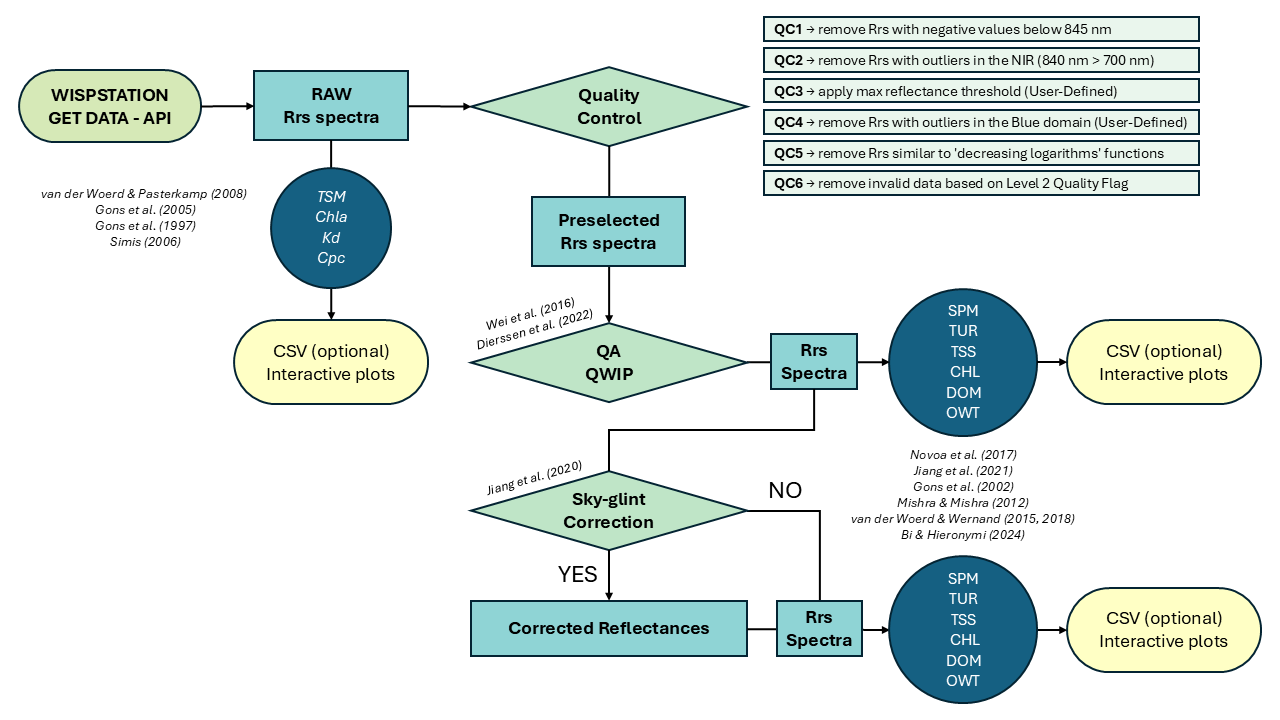
\includegraphics[width=1\linewidth,height=\textheight,keepaspectratio]{Figure_1.png}
\caption{\emph{WISP.data workflow.}}\label{fig:workflow}
\end{figure}

The package architecture is organized into functional modules:

\begin{itemize}
\tightlist
\item
  \textbf{Data Integration Layer}: the functions
  \texttt{wisp\_get\_reflectance\_data()} and its iterative wrapper
  \texttt{wisp\_get\_reflectance\_multi\_data()} manage the
  communication with the Water Insight API using the \texttt{httr2}
  framework. These functions allow users to filter measurements by
  specific dates and time periods. Raw JSON/text responses are parsed,
  unnested, and converted into structured \texttt{tibble} objects. This
  layer also handles the transformation of spectral columns into a
  standardized format, making the data immediately ready for analysis.
\item
  \textbf{Physical Awareness}: \texttt{WISP.data} integrates the
  \texttt{units} package to maintain physical consistency. Every
  measurement retrieved is assigned its proper unit, preventing
  dimensional errors in downstream calculations.
\item
  \textbf{Modular Quality Control (QC)}: the
  \texttt{wisp\_qc\_reflectance\_data()} function implements a
  multi-step diagnostic pipeline, allowing for a sequential execution of
  six distinct QC tests (QC1--QC6) alongside advanced validation metrics
  like Quality Assurance (QA) (Wei, Lee, and Shang 2016) and Quality
  Water Index Polynomial (QWIP) (Dierssen et al. 2022). The architecture
  is highly parameterized, enabling researchers to tune thresholds
  (e.g., \texttt{maxPeak}, \texttt{maxPeak\_blue},
  \texttt{qa\_threshold}, and \texttt{qwip\_threshold}) to suit specific
  optical water types, from oligotrophic to highly turbid and productive
  environments.
\item
  \textbf{Sky-glint removal (SR)}: the
  \texttt{wisp\_sr\_reflectance\_data()} function implements a sky-glint
  removal algorithm based on the methodology proposed by Jiang,
  Matsushita, and Yang (2020).
\item
  \textbf{Application of third-party algorithms}: \texttt{WISP.data}
  currently supports a wide array of standardized algorithms for
  assessing the physical and optical properties of water (Lee, Carder,
  and Arnone 2002; van der Woerd and Wernand 2015, 2018; Bi and
  Hieronymi 2024) and for estimating the concentrations of water quality
  parameters (Gons 1999; Gons, Rijkeboer, and Ruddick 2002; Nechad,
  Ruddick, and Park 2010; Mishra and Mishra 2012; Novoa et al. 2017;
  Jiang et al. 2021). These are implemented as modular flags within
  \texttt{wisp\_qc\_reflectance\_data()} and
  \texttt{wisp\_sr\_reflectance\_data()} functions, allowing for a
  seamless ``one-call'' workflow from native spectra to validated
  products.
\item
  \textbf{Visualization layer}: utilizing \texttt{ggplot2} and
  \texttt{plotly} as backends, the package provides consistent
  visualization interfaces. Functions like
  \texttt{wisp\_plot\_reflectance\_data()},
  \texttt{wisp\_plot\_comparison()} (Figure \ref{fig:spectra}), and
  \texttt{wisp\_trend\_plot()} (Figures \ref{fig:trendsingle},
  \ref{fig:trendmulti}) are designed to handle both publication-quality
  plots and interactive exploration.
\end{itemize}

\begin{figure}
\centering
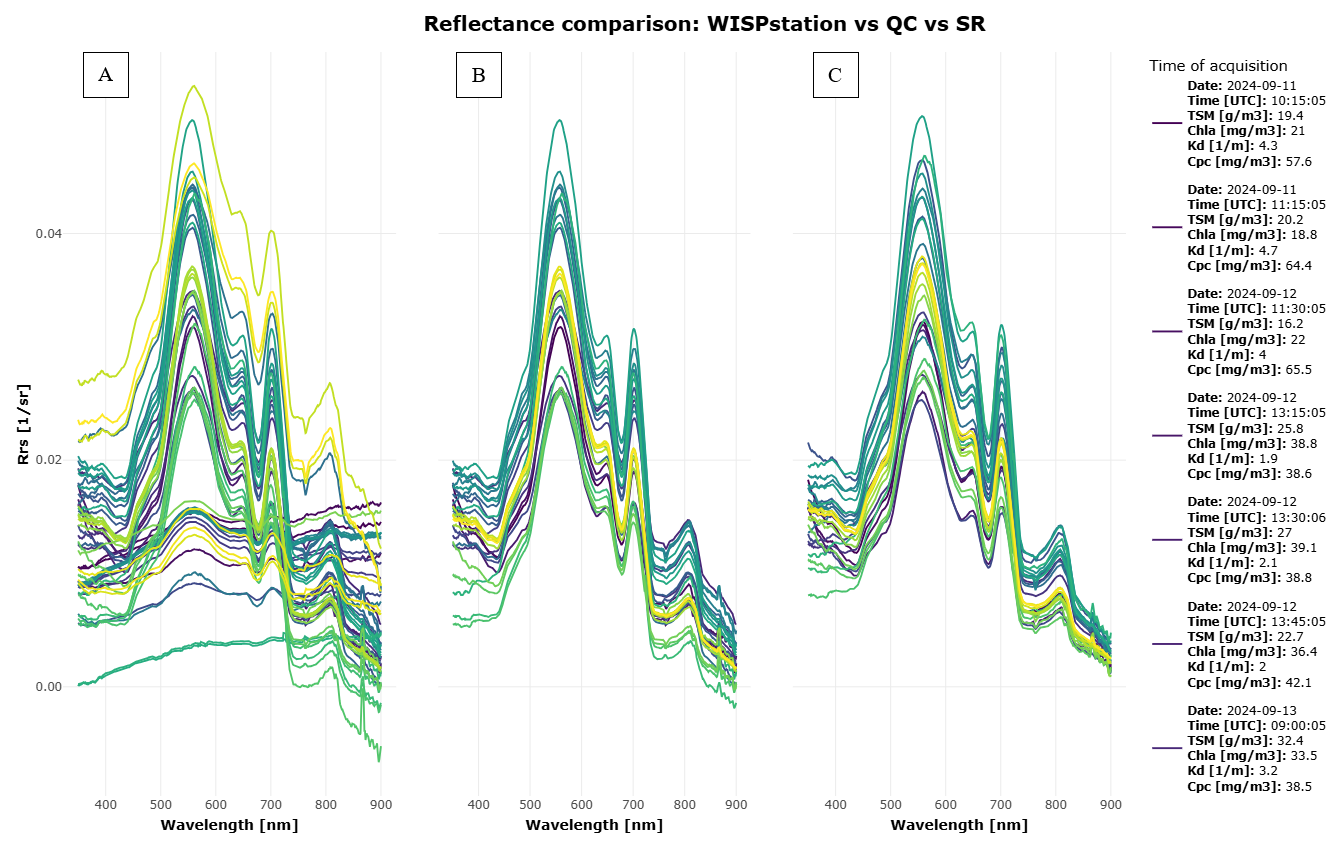
\includegraphics[width=1\linewidth,height=\textheight,keepaspectratio]{Figure_2.png}
\caption{\emph{Plot resulting from the \texttt{wisp\_plot\_comparison()}
function showing the comparison between: A) native WISPstation
R\textsubscript{rs}, B) R\textsubscript{rs} filtered by ``QC'', C)
R\textsubscript{rs} to which ``SR'' has been applied (site: Trasimeno;
period: 11/09/2024 -- 17/09/2024).}}\label{fig:spectra}
\end{figure}

\begin{figure}
\centering
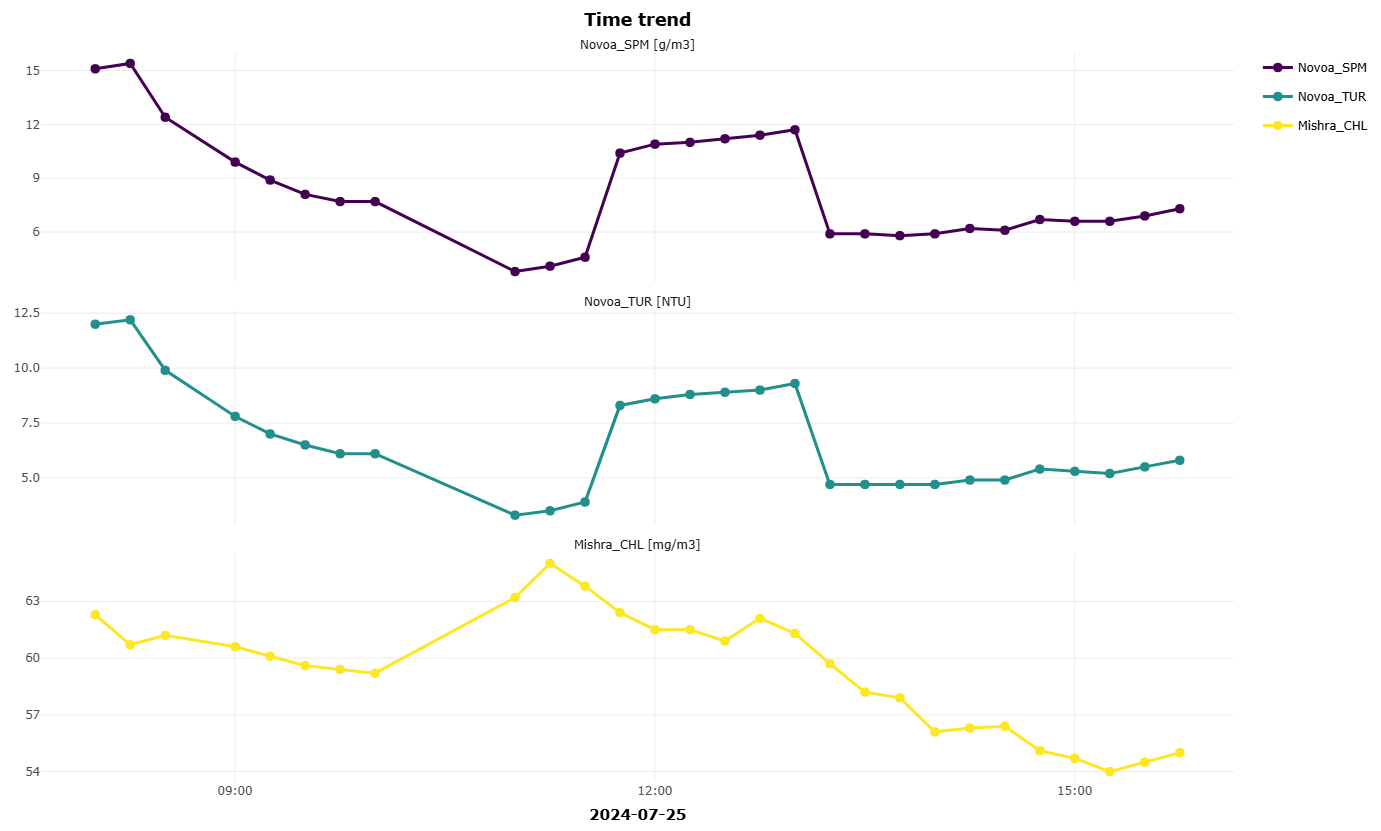
\includegraphics[width=1\linewidth,height=\textheight,keepaspectratio]{Figure_3.png}
\caption{\emph{Plot resulting from the \texttt{wisp\_trend\_plot()}
function showing the temporal trend of three exemplary parameters (from
top to bottom: ``Novoa\_SPM'', ``Novoa\_TUR'', and ``Mishra\_CHL'') for
25/07/2024 from 8 a.m. to 4 p.m. (site:
Trasimeno).}}\label{fig:trendsingle}
\end{figure}

\begin{figure}
\centering
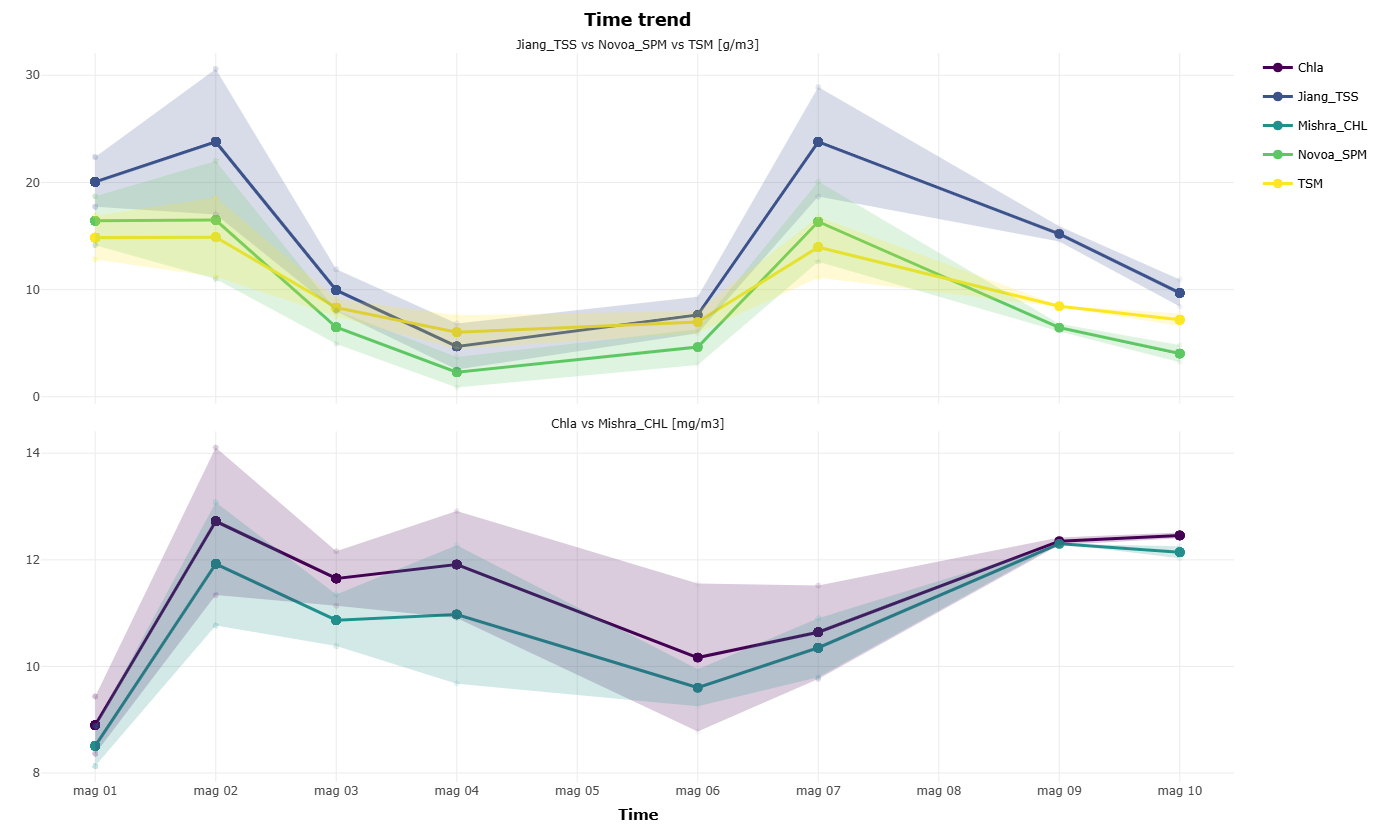
\includegraphics[width=1\linewidth,height=\textheight,keepaspectratio]{Figure_4.png}
\caption{\emph{Plot resulting from the \texttt{wisp\_trend\_plot()}
function showing the temporal trend of five exemplary parameters
averaged on a daily basis: in the upper plot, a comparison between the
WISPstation native algorithm (TSM) and two third-party algorithms for
estimating suspended solids concentration (``Novoa\_SPM'' and
``Jiang\_TSS''); in the lower plot, the comparison between the
WISPstation native chlorophyll-a algorithm (Chla) and Mishra\_CHL
algorithm. (site: Trasimeno; period: 01/05/2024 --
10/05/2024).}}\label{fig:trendmulti}
\end{figure}

\section{Research impact statement}\label{research-impact-statement}

The package was successfully tested using two WISPstations installed in
two different aquatic environments in Italy. The first was installed in
April 2018 in Lake Trasimeno, on a lake platform located approximately
400 m from Polvese Island (43.122° N, 12.134° E). The second was
deployed in September 2024 along the Po River at Pontelagoscuro (44.889°
N, 11.6106° E), approximately 95 km upstream from its confluence with
the northern Adriatic Sea, on a floating monitoring platform operated by
the Agenzia Interregionale per il fiume Po (AIPO).

Lake Trasimeno, located in central Italy, is the fourth-largest lake in
the country (124 km\textsuperscript{2}). Its catchment is characterized
by intensive agricultural practices and livestock farming, which lead to
significant nutrient loading. These conditions frequently promote
phytoplankton blooms, including potentially harmful cyanobacteria. The
lake exhibits complex hydrodynamic behavior, with strong intra-day and
inter-day variability driven by meteorological forcing such as
temperature fluctuations and wind-induced sediment resuspension. The Po
River, the longest river in Italy, flows across the Po Valley and
governs the exchanges at the river--sea interface, driving the transfer
of sediments, nutrients, and organic matter toward the northern Adriatic
Sea and influencing coastal biogeochemistry and water quality. The river
is characterized by highly dynamic hydrological conditions, with
discharge variability driven by seasonal cycles as well as extreme
events such as floods and prolonged drought periods. These conditions
strongly affect sediment transport and turbidity, resulting in rapid
changes in water optical properties.

Both environments are the focus of long-standing research efforts aimed
at understanding the spatio-temporal dynamics of parameters that can
also be monitored through remote sensing. The stations are designated
research sites within ESFRI Research Infrastructures. Particularly, Lake
Trasimeno\footnote{\url{https://elter-ri.eu}} is part of the Integrated
European Long-Term Ecosystem, Critical Zone and Socio-Ecological
Research (eLTER RI), while the Po River\footnote{\url{https://danubius-ri.eu}}
is a Supersite of DANUBIUS-RI, the International Centre for Advanced
Studies on River-Sea Systems, a pan-European distributed Research
Infrastructure enabling integrated studies of rivers and their
catchments, transitional waters such as estuaries, deltas and lagoons,
and their adjacent coastal seas.

Within these RIs, the availability of continuous, comparable, and
quality-controlled measurements is essential to minimize uncertainties
and ensure data reliability. Such measurements, acquired through
high-quality sensor systems and complemented by parameters derived from
robust algorithms, can be particularly valuable for the calibration and
validation (Cal/Val) of satellite-derived products. Within eLTER RI,
these measurements contribute to the definition of standardized
variables (Zacharias et al. 2026), known as Standard Observations (SOs),
which integrate target variables, measurement methods, and protocols to
ensure harmonized data collection across sites at the continental scale.
Among these, the SO ``Phenological traits -- SOBIO\_15'' specifically
addresses the use of remote sensing approaches for monitoring vegetation
phenological dynamics, including in aquatic ecosystems, encompassing
both inland standing waters (lakes) and running waters (rivers).

The scientific utility of \texttt{WISP.data} has recently been
demonstrated by Ghirardi et al.~(under review), who investigated the
spatio-temporal dynamics of suspended particulate matter and
chlorophyll-a in Lake Trasimeno using a synergistic approach. By
combining high-frequency in situ observations processed with
\texttt{WISP.data} and multisensor satellite imagery (2019--2024), the
study validated R\textsubscript{rs} products from 14 different satellite
sensors. The strong agreement between satellite-derived estimates and
the \texttt{WISP.data} processed ground-truth enabled the accurate
retrieval of both water quality parameters. These results highlight the
package's role in bridging the gap between local autonomous measurements
and large-scale satellite monitoring, facilitating the study of rapid
environmental changes in lake ecosystems. For the Po River,
\texttt{WISP.data} is used to process high-frequency hyperspectral
radiometric data collected at the Pontelagoscuro platform, including
quality control, sky-glint correction, and the application of algorithms
to derive turbidity from optical measurements. The resulting time series
of above-water observations supports the assessment of hyperspectral and
multispectral satellite missions, enabling the testing of different
atmospheric correction algorithms. In addition, water turbidity derived
from WISPstation measurements is compared with in situ data acquired by
in-water turbidimeters, enabling consistency evaluation between
radiometric-derived and direct observations. This integrated approach
enhances the interpretation of turbidity dynamics in highly variable
riverine systems.

Looking ahead, the modular architecture of \texttt{WISP.data} is
well-suited to be extended and adapted to other optical view fixed
spectroradiometric systems widely used in the scientific community for
water body monitoring, thereby promoting greater interoperability and
standardization in the processing of in situ optical data.

\section{AI usage disclosure}\label{ai-usage-disclosure}

No generative AI tools were used in the writing of this manuscript, or
the preparation of supporting materials. Generative AI tools were used
as a support for code development.

\section{Acknowledgements}\label{acknowledgements}

The development of this package and the related publication has been
funded by the European Union -- Next Generation EU, Mission 4, Component
2 -- CUP B53C22002150006, within the Project IR0000032 -- ITINERIS
(Italian Integrated Environmental Research Infrastructures System), and
has been partially supported by the European Union's Horizon 2020
research and innovation programme under the H2020 eLTER‑Plus project
(Grant Agreement No.~871128, DOI: 10.3030/871128) and the eLTER EnRich
project (Grant Agreement No.~101131751, DOI: 10.3030/101131751).

\section*{References}\label{references}
\addcontentsline{toc}{section}{References}

\protect\phantomsection\label{refs}
\begin{CSLReferences}{1}{0}
\bibitem[\citeproctext]{ref-hyperSpec}
Beleites, C., A. Bonifacio, M. Dahms, B. Egert, S. Fuller, V. Gegzna, R.
Guliev, et al. 2024. \emph{{hyperSpec: a package to handle hyperspectral
data sets in R}}. \url{https://r-hyperspec.github.io/hyperSpec}.

\bibitem[\citeproctext]{ref-Bi:2024}
Bi, S., and M. Hieronymi. 2024. {``{Holistic optical water type
classification for ocean, coastal, and inland waters}.''}
\emph{Limnology and Oceanography} 69 (7): 1547--61.
\url{https://doi.org/10.1002/lno.12606}.

\bibitem[\citeproctext]{ref-Bresciani:2020}
Bresciani, M., M. Pinardi, G. Free, G. Luciani, S. Ghebrehiwot, M.
Laanen, S. Peters, V. Della Bella, R. Padula, and C. Giardino. 2020.
{``{The Use of Multisource Optical Sensors to Study Phytoplankton
Spatio-Temporal Variation in a Shallow Turbid Lake}.''} \emph{Water} 12
(1): 284. \url{https://doi.org/10.3390/w12010284}.

\bibitem[\citeproctext]{ref-Dierssen:2022}
Dierssen, H. M., R. A. Vandermeulen, B. B. Barnes, A. Castagna, E.
Knaeps, and Q. Vanhellemont. 2022. {``{QWIP: A quantitative metric for
quality control of aquatic reflectance spectral shape using the apparent
visible wavelength}.''} \emph{Frontiers in Remote Sensing} 3: 869611.
\url{https://doi.org/10.3389/frsen.2022.869611}.

\bibitem[\citeproctext]{ref-Free:2021}
Free, G., M. Bresciani, M. Pinardi, C. Giardino, K. Alikas, K. Kangro,
E. I. Rõõm, et al. 2021. {``{Detecting Climate Driven Changes in
Chlorophyll-a Using High Frequency Monitoring: The Impact of the 2019
European Heatwave in Three Contrasting Aquatic Systems}.''}
\emph{Sensors} 21 (18): 6242. \url{https://doi.org/10.3390/s21186242}.

\bibitem[\citeproctext]{ref-Gons:1999}
Gons, H. J. 1999. {``{Optical teledetection of chlorophyll a in turbid
inland waters}.''} \emph{Environmental Science \& Technology} 33 (7):
1127--32. \url{https://doi.org/10.1021/es9809657}.

\bibitem[\citeproctext]{ref-Gons:1997}
Gons, H. J., J. Ebert, and J. Kromkamp. 1997. {``Optical Teledetection
of the Vertical Attenuation Coefficient for Downward Quantum Irradiance
of Photosynthetically Available Radiation in Turbid Inland Waters.''}
\emph{Aquatic Ecology} 31 (3): 299--311.
\url{https://doi.org/10.1023/A:1009924823521}.

\bibitem[\citeproctext]{ref-Gons:2002}
Gons, H. J., M. Rijkeboer, and K. G. Ruddick. 2002. {``{A
chlorophyll-retrieval algorithm for satellite imagery (Medium Resolution
Imaging Spectrometer) of inland and coastal waters}.''} \emph{Journal of
Plankton Research} 24 (9): 947--51.
\url{https://doi.org/10.1093/plankt/24.9.947}.

\bibitem[\citeproctext]{ref-Gons:2005}
---------. 2005. {``{Effect of a waveband shift on chlorophyll retrieval
from MERIS imagery of inland and coastal waters}.''} \emph{Journal of
Plankton Research} 27 (1): 125--27.
\url{https://doi.org/10.1093/plankt/fbh151}.

\bibitem[\citeproctext]{ref-Hommersom:2012}
Hommersom, A., S. Kratzer, M. L. Laanen, I. Ansko, M. Ligi, M.
Bresciani, and S. W. M. Peters. 2012. {``{Intercomparison in the field
between the new WISP-3 and other radiometers (TriOS Ramses, ASD
FieldSpec, and TACCS)}.''} \emph{Journal of Applied Remote Sensing} 6
(1): 063615. \url{https://doi.org/10.1117/1.JRS.6.063615}.

\bibitem[\citeproctext]{ref-Jiang:2021}
Jiang, D., B. Matsushita, N. Pahlevan, D. Gurlin, M. K. Lehmann, C. G.
Fichot, and D. O'Donnell. 2021. {``{Remotely estimating total suspended
solids concentration in clear to extremely turbid waters using a novel
semi-analytical method}.''} \emph{Remote Sensing of Environment} 258:
112386. \url{https://doi.org/10.1016/j.rse.2021.112386}.

\bibitem[\citeproctext]{ref-Jiang:2020}
Jiang, D., B. Matsushita, and W. Yang. 2020. {``{A simple and effective
method for removing residual reflected skylight in above-water remote
sensing reflectance measurements}.''} \emph{ISPRS Journal of
Photogrammetry and Remote Sensing} 165: 16--27.
\url{https://doi.org/10.1016/j.isprsjprs.2020.05.003}.

\bibitem[\citeproctext]{ref-Lee:2002}
Lee, Z., K. L. Carder, and R. A. Arnone. 2002. {``{Deriving inherent
optical properties from water color: a multiband quasi-analytical
algorithm for optically deep waters}.''} \emph{Applied Optics} 41 (27):
5755--72. \url{https://doi.org/10.1364/AO.41.005755}.

\bibitem[\citeproctext]{ref-Mishra:2012}
Mishra, S., and D. R. Mishra. 2012. {``{Normalized difference
chlorophyll index: A novel model for remote estimation of chlorophyll-a
concentration in turbid productive waters}.''} \emph{Remote Sensing of
Environment} 117: 394--406.
\url{https://doi.org/10.1016/j.rse.2011.10.016}.

\bibitem[\citeproctext]{ref-Nechad:2010}
Nechad, B., K. G. Ruddick, and Y. Park. 2010. {``{Calibration and
validation of a generic multisensor algorithm for mapping of total
suspended matter in turbid waters}.''} \emph{Remote Sensing of
Environment} 114 (4): 854--66.
\url{https://doi.org/10.1016/j.rse.2009.11.022}.

\bibitem[\citeproctext]{ref-Novoa:2017}
Novoa, S., D. Doxaran, A. Ody, Q. Vanhellemont, V. Lafon, B. Lubac, and
P. Gernez. 2017. {``{Atmospheric corrections and multi-conditional
algorithm for multi-sensor remote sensing of suspended particulate
matter in low-to-high turbidity levels coastal waters}.''} \emph{Remote
Sensing} 9 (1): 61. \url{https://doi.org/10.3390/rs9010061}.

\bibitem[\citeproctext]{ref-cops}
Rusch, T., and P. Mair. 2024. \emph{{cops: Cluster Optimized Proximity
Scaling}}. \url{https://doi.org/10.32614/CRAN.package.cops}.

\bibitem[\citeproctext]{ref-cops-paper}
Rusch, T., P. Mair, and K. Hornik. 2021. {``{Cluster Optimized Proximity
Scaling}.''} \emph{Journal of Computational and Graphical Statistics} 30
(4): 1156--67. \url{https://doi.org/10.1080/10618600.2020.1869027}.

\bibitem[\citeproctext]{ref-Simis:2006}
Simis, S. G. H. 2006. {``Blue-Green Catastrophe: Remote Sensing of Mass
Viral Lysis of Cyanobacteria.''} PhD thesis, Amsterdam, Netherlands:
Vrije Universiteit Amsterdam.
\url{https://scholarlypublications.universiteitleiden.nl/handle/1887/11019}.

\bibitem[\citeproctext]{ref-vanderWoerd:2008}
van der Woerd, H. J., and R. Pasterkamp. 2008. {``{HYDROPT: A fast and
flexible method to retrieve chlorophyll-a from multispectral satellite
observations of optically complex coastal waters}.''} \emph{Remote
Sensing of Environment} 112 (4): 1795--1807.
\url{https://doi.org/10.1016/j.rse.2007.09.001}.

\bibitem[\citeproctext]{ref-vanderWoerd:2015}
van der Woerd, H. J., and M. R. Wernand. 2015. {``{True colour
classification of natural waters with medium-spectral resolution
satellites: SeaWiFS, MODIS, MERIS and OLCI}.''} \emph{Sensors} 15 (10):
25663--80. \url{https://doi.org/10.3390/s151025663}.

\bibitem[\citeproctext]{ref-vanderWoerd:2018}
---------. 2018. {``{Hue-angle product for low to medium spatial
resolution optical satellite sensors}.''} \emph{Remote Sensing} 10 (2):
180. \url{https://doi.org/10.3390/rs10020180}.

\bibitem[\citeproctext]{ref-Wei:2016}
Wei, J., Z. Lee, and S. Shang. 2016. {``{A system to measure the data
quality of spectral remote-sensing reflectance of aquatic
environments}.''} \emph{Journal of Geophysical Research: Oceans} 121
(11): 8189--8207. \url{https://doi.org/10.1002/2016JC012126}.

\bibitem[\citeproctext]{ref-Zacharias:2026}
Zacharias, S., T. Lumpi, J. Weldon, T. Dirnboeck, J. Gaillardet, P.
Haase, and M Mirtl. 2026. {``Achieving Harmonized and Integrated
Long-Term Environmental Observation of Essential Ecosystem Variables --
Elter's Framework of Standard Observations.''} \emph{Earth's Future}.
\url{https://doi.org/10.1029/2025EF006743}.

\end{CSLReferences}

\end{document}
